\documentclass[11pt,a4paper]{article}
\usepackage[margin=2.3cm]{geometry}
\usepackage{amsmath,amssymb}
\usepackage{booktabs}
\usepackage{graphicx}
\usepackage{subcaption}
\usepackage[font=small,labelfont=bf]{caption}
\usepackage{xcolor}
\usepackage{microtype}
\usepackage{enumitem}
\usepackage[colorlinks=true,linkcolor=blue!45!black,citecolor=blue!45!black]{hyperref}
\usepackage{titlesec}
\titleformat{\section}{\normalfont\Large\bfseries\color{blue!30!black}}{\thesection}{1em}{}
\titleformat{\subsection}{\normalfont\large\bfseries\color{blue!35!black}}{\thesubsection}{1em}{}
\setlength{\parskip}{4pt}
\setlength{\parindent}{0pt}
\newcommand{\vs}{\sigma^2}

\title{\bfseries In-context unlearning:\\ membership AUC under prompt-time corruption\\
\large Stage 1 --- the AUC vs.\ $\mathrm{Var}(\epsilon)$ sweep}
\author{}
\date{30 July 2026}

\begin{document}
\maketitle
\vspace{-2.2em}

\begin{abstract}
\noindent
We measure whether corrupting a forget example \emph{in the prompt} removes the
membership evidence a shadow-model attacker can extract. Three corruption
families from the brief are swept across four decades of noise variance on four
configurations, with 512 shadow models per hypothesis and nine independent
seed combinations per point. Three results. First, the measured AUC agrees with
an independently derived closed form to $4\times10^{-4}$, which validates the
pipeline end to end. Second, the movement toward chance is almost entirely
\emph{masking} --- added variance --- rather than removal, at every corruption
strength below $\vs\approx1$. Third, and most consequential, reaching
chance costs a factor of ${\sim}2400$ in preservation error: within the swept
range there is no operating point at which the attacker is defeated and the
model is preserved. The arms also separate cleanly by which moment of the score
distribution they move: the zero-mean input-noise arm can only approach chance,
whereas the deterministic label flip carries a mean shift with no variance and
overshoots \emph{past} it. Finally, a negative control: equalising the
group covariance spectra does \emph{not} return the baseline AUC to chance,
so the signal is not an artefact of one group being intrinsically harder.
\end{abstract}


\section{Setup}

A linear-attention model reads a query $x_q$, a retain set $\mathcal{D}_r$, and
a corrupted forget set $\widetilde{\mathcal{D}}_f$ in context. Targets are
linear in a task vector drawn afresh per sequence,
$y = \omega^{\!\top} x$, so the model must infer $\omega$ from the context
rather than memorise it. Because the model is linear in the context, the whole
ensemble reduces to one read-out matrix $M$ per shadow, and a shadow ensemble of
512 trains in seconds.

\paragraph{Corruption families.} The forget tokens are edited at prompt time,
with no weight update:
\begin{align*}
\text{C1} &: (x_f,\,y_f) \to (x_f,\ y_f+\epsilon), &&\epsilon\sim\mathcal{N}(0,\vs)\\
\text{C2} &: (x_f,\,y_f) \to (x_f+\epsilon,\ y_f), &&\epsilon\sim\mathcal{N}(0,\vs I_D)\\
\text{C3} &: (x_f,\,y_f) \to (x_f+\epsilon_1,\ y_f+\epsilon_2), &&\epsilon_1\perp\epsilon_2
\end{align*}
plus a deterministic label flip $y_f\to(1-2t)y_f$ and an input-whitening arm
that maps the forget covariance toward the retain covariance.

\paragraph{The attacker.} Membership inference over the \emph{model} axis at a
fixed probe point: $H_1$ is the fully trained model after the in-context edit,
$H_0$ is an oracle retrained without the forget group. The statistic is the
sign-aligned residual $\mathrm{sign}(y)\,(\hat y - y)$, ranked across the shadow
axis by Mann--Whitney and averaged over 64 probe points. Success is
$\mathrm{AUC}\to 0.5$.

\paragraph{Two conventions that matter.} Both hypotheses are scored on the
\emph{same} corrupted prompt with the same noise draw. Scoring the oracle on a
clean prompt instead lets a distinguisher win by detecting that an edit
occurred at all, and that confound grows with the very axis being plotted.
Separately, each point is repeated with a single noise draw broadcast across all
shadows; comparing against the per-shadow draw isolates how much of any AUC
movement is variance inflation rather than information removal.


\section{Configurations}

All four configurations give the three groups the \emph{same} covariance
spectrum, so no group is intrinsically harder than another and the usual
difficulty confound is unavailable. They differ in how anisotropic that shared
spectrum is (participation ratio $\mathrm{PR}$, where $\mathrm{PR}=1$ is a
needle and $\mathrm{PR}=D=4$ a sphere) and in whether each group is rotated into
its own eigenbasis.


\begin{table}[h]\centering\small
\begin{tabular}{lccccccc}
\toprule
configuration & PR (all groups) & basis & $D$ & $N$ & shadows & seed combos & rows \\
\midrule
\texttt{rot\_mid\_identity} & 2.65 & identity & 4 & 31 & 512 & 9 & 1440 \\
\texttt{rot\_flat\_identity} & 3.55 & identity & 4 & 31 & 512 & 9 & 1440 \\
\texttt{rot\_mid} & 2.65 & random & 4 & 31 & 512 & 9 & 1440 \\
\texttt{rot\_flat} & 3.55 & random & 4 & 31 & 512 & 9 & 1440 \\
\bottomrule
\end{tabular}
\caption{The four configurations. The two \emph{identity} rows are nulls: with
one spectrum and one basis the three groups are literally the same
distribution, so the full and oracle models train on indistinguishable data and
the AUC must be chance. They are a correctness test on the pipeline, not an
experiment.}
\end{table}


\section{Results}
\subsection{The nulls pass}


\begin{table}[h]\centering\small
\begin{tabular}{lcccc}
\toprule
& \multicolumn{2}{c}{ATTN-M} & \multicolumn{2}{c}{ATTN-S}\\
\cmidrule(lr){2-3}\cmidrule(lr){4-5}
configuration & AUC & across-seed range & AUC & across-seed range \\
\midrule
\texttt{rot\_mid\_identity} & 0.5025 & 0.5012--0.5046 & 0.5041 & 0.5012--0.5069 \\
\texttt{rot\_flat\_identity} & 0.5008 & 0.4979--0.5036 & 0.5000 & 0.4982--0.5021 \\
\texttt{rot\_mid} & \textbf{0.4174} & 0.4171--0.4180 & \textbf{0.4292} & 0.4247--0.4320 \\
\texttt{rot\_flat} & \textbf{0.4482} & 0.4477--0.4489 & \textbf{0.4680} & 0.4660--0.4702 \\
\bottomrule
\end{tabular}
\caption{Membership AUC at zero corruption. The two null configurations sit at
chance, confirming that the two hypotheses are not coupled anywhere in the
training or evaluation code.}
\end{table}

\subsection{The baseline signal survives equalised spectra}

The two rotated configurations are the result, and they are a negative one. All
three groups share a spectrum, so every group is equally hard; yet the AUC sits
0.07--0.08 from chance. The across-seed range is $0.0009$ wide for
\texttt{rot\_mid} ATTN-M --- three independent training runs agreeing to
the fourth decimal. This is systematic, not sampling noise.

This was predicted to go the other way. The expectation recorded before the run
was that equalising the spectra would largely cancel the read-out mismatch
between the two hypotheses and drive AUC toward chance. It does not, and the
prediction is recorded as failed. A simulation containing \emph{no} memorisation
--- both models replaced by the idealised preconditioner
$\Lambda_{\text{train}}^{-1}$ for the groups each trained on --- predicts
$0.313$ for \texttt{rot\_mid} against $0.417$ measured: the right sign
and rough magnitude, over-predicting the confound. Decomposing the residual
into read-out mismatch versus genuine memorisation is the main open question
and requires the read-out covectors from the trained ensembles.


\subsection{The sweeps}

\begin{figure}[h]\centering
\begin{subfigure}{0.49\textwidth}\includegraphics[width=\linewidth]{fig/auc_C1_rot_mid.pdf}
\caption{C1, label noise}\end{subfigure}\hfill
\begin{subfigure}{0.49\textwidth}\includegraphics[width=\linewidth]{fig/auc_C2_rot_mid.pdf}
\caption{C2, input noise}\end{subfigure}\\[4pt]
\begin{subfigure}{0.49\textwidth}\includegraphics[width=\linewidth]{fig/auc_C3_rot_mid.pdf}
\caption{C3, both}\end{subfigure}\hfill
\begin{subfigure}{0.49\textwidth}\includegraphics[width=\linewidth]{fig/auc_flip_rot_mid.pdf}
\caption{deterministic label flip}\end{subfigure}
\caption{Membership AUC against corruption strength on \texttt{rot\_mid}.
Bands are the min--max range across nine (training seed, probe seed)
combinations, not a within-run bootstrap. The thin dark line under C1 and C2 is
the closed-form prediction. The three Gaussian arms rise toward chance and stop;
the deterministic flip (d) rises \emph{through} chance and keeps going. Section
3.6 explains why.}
\end{figure}

\begin{figure}[h]\centering
\begin{subfigure}{0.49\textwidth}\includegraphics[width=\linewidth]{fig/auc_C1_rot_flat.pdf}
\caption{C1 on \texttt{rot\_flat}}\end{subfigure}\hfill
\begin{subfigure}{0.49\textwidth}\includegraphics[width=\linewidth]{fig/auc_C2_rot_flat.pdf}
\caption{C2 on \texttt{rot\_flat}}\end{subfigure}\\[4pt]
\begin{subfigure}{0.49\textwidth}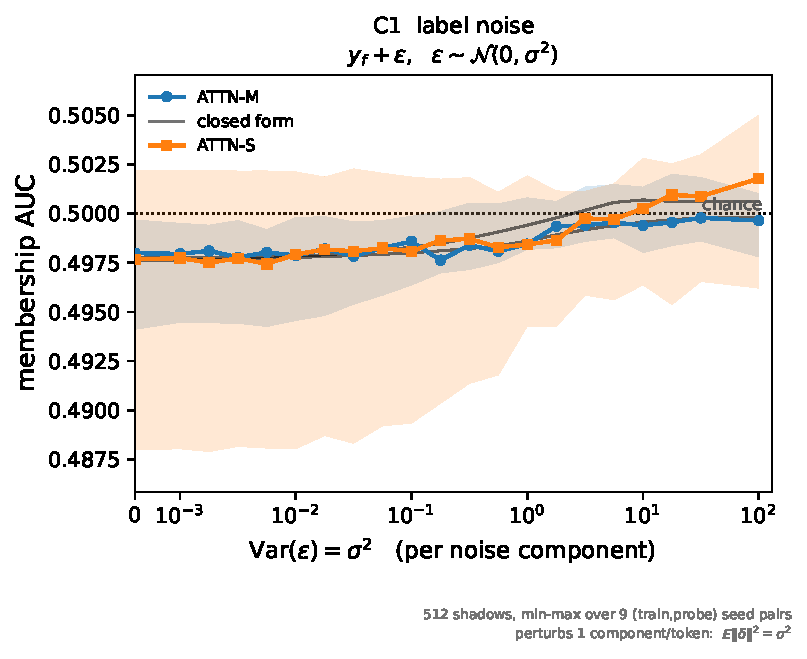
\includegraphics[width=\linewidth]{fig/auc_C1_rot_mid_identity.pdf}
\caption{C1 on the null}\end{subfigure}\hfill
\begin{subfigure}{0.49\textwidth}\includegraphics[width=\linewidth]{fig/auc_C2_rot_mid_identity.pdf}
\caption{C2 on the null}\end{subfigure}
\caption{The same sweeps on the flatter configuration and on a null. The null
panels are flat at chance across the entire grid, which is what a corruption
sweep should look like when there is nothing to remove.}
\end{figure}


\clearpage
\subsection{The closed form is exact}

Because the read-out is linear in the context, the effect of Gaussian context
noise is available analytically. Writing $c = M^{\!\top}t_q = [c_x; c_y]$ and
$u=\sum_i t_i y_i$ with $t_i=[x_i;y_i]$, the last coordinate of $u$ is
$\sum_i y_i^2$ --- the label enters \emph{quadratically}. Hence
\[
\text{C1}:\quad \mathbb{E}[\Delta\hat y] = \frac{c_y\, n_f\, \vs}{N+1},
\qquad
\text{C2}:\quad \mathbb{E}[\Delta\hat y] = 0 .
\]
C2 is exactly zero-mean; C1 is not, because the $\epsilon^2$ term survives
expectation in the label--label block. Feeding these moments through a Gaussian
approximation of the score distribution gives a predicted AUC with no free
parameters.


\begin{table}[h]\centering\small
\begin{tabular}{lllcc}
\toprule
configuration & architecture & arm & mean $|$error$|$ & max $|$error$|$ \\
\midrule
\texttt{rot\_mid} & ATTN-M & C1 & 0.00048 & 0.00176 \\
\texttt{rot\_mid} & ATTN-M & C2 & 0.00039 & 0.00163 \\
\texttt{rot\_mid} & ATTN-S & C1 & 0.00045 & 0.00199 \\
\texttt{rot\_mid} & ATTN-S & C2 & 0.00034 & 0.00140 \\
\texttt{rot\_flat} & ATTN-M & C1 & 0.00040 & 0.00180 \\
\texttt{rot\_flat} & ATTN-M & C2 & 0.00032 & 0.00147 \\
\texttt{rot\_flat} & ATTN-S & C1 & 0.00044 & 0.00188 \\
\texttt{rot\_flat} & ATTN-S & C2 & 0.00036 & 0.00153 \\
\bottomrule
\end{tabular}
\caption{Absolute difference between the predicted and measured AUC over the
whole grid. Agreement at $4\times10^{-4}$ means the simulation and the algebra
are independently confirming each other. A systematic gap would have localised a
bug in one of them.}
\end{table}



\subsection{The two channels, separated}

The arms differ in \emph{which} moment of the score distribution they move, and
the sweeps separate the two cleanly.


\begin{table}[h]\centering\small
\begin{tabular}{lllcccc}
\toprule
configuration & arch & arm & min AUC & max AUC & crosses $0.5$? & at \\
\midrule
\texttt{rot\_mid} & ATTN-M & C1 & 0.4273 & 0.4974 & no &  \\
\texttt{rot\_mid} & ATTN-M & C2 & 0.4273 & 0.4975 & no &  \\
\texttt{rot\_mid} & ATTN-M & C3 & 0.4273 & 0.4978 & no &  \\
\texttt{rot\_mid} & ATTN-M & flip & 0.4272 & 0.5331 & \textbf{yes} & 0.9 \\
\texttt{rot\_mid} & ATTN-M & whiten & 0.4273 & 0.4394 & no &  \\
\texttt{rot\_mid} & ATTN-S & C1 & 0.4310 & 0.4972 & no &  \\
\texttt{rot\_mid} & ATTN-S & C2 & 0.4310 & 0.4971 & no &  \\
\texttt{rot\_mid} & ATTN-S & C3 & 0.4310 & 0.4977 & no &  \\
\texttt{rot\_mid} & ATTN-S & flip & 0.4308 & 0.5248 & \textbf{yes} & 1 \\
\texttt{rot\_mid} & ATTN-S & whiten & 0.4310 & 0.4398 & no &  \\
\texttt{rot\_flat} & ATTN-M & C1 & 0.4463 & 0.4988 & no &  \\
\texttt{rot\_flat} & ATTN-M & C2 & 0.4463 & 0.4989 & no &  \\
\texttt{rot\_flat} & ATTN-M & C3 & 0.4463 & 0.4989 & no &  \\
\texttt{rot\_flat} & ATTN-M & flip & 0.4448 & 0.5143 & \textbf{yes} & 1 \\
\texttt{rot\_flat} & ATTN-M & whiten & 0.4463 & 0.4532 & no &  \\
\texttt{rot\_flat} & ATTN-S & C1 & 0.4650 & 0.4972 & no &  \\
\texttt{rot\_flat} & ATTN-S & C2 & 0.4651 & 0.4989 & no &  \\
\texttt{rot\_flat} & ATTN-S & C3 & 0.4651 & 0.4984 & no &  \\
\texttt{rot\_flat} & ATTN-S & flip & 0.4646 & 0.5074 & \textbf{yes} & 1 \\
\texttt{rot\_flat} & ATTN-S & whiten & 0.4651 & 0.4690 & no &  \\
\bottomrule
\end{tabular}
\caption{Range of the AUC curve for every arm. Only the deterministic flip
crosses chance, and it does so in all four cases.}
\end{table}

The pattern follows directly from the algebra. Write the predicted AUC as
$\Phi\!\big((\mu_1-\mu_0)/\sqrt{v_1+v_0}\big)$ and note that corruption can move
the numerator, the denominator, or both:

\begin{itemize}[leftmargin=1.4em,itemsep=1pt]
\item \textbf{C2} is \emph{exactly} zero-mean. It can only inflate the
denominator, so it drives AUC toward $0.5$ and mathematically cannot cross.
\item \textbf{flip} is deterministic given the probe: it carries a mean shift
and \emph{no} variance at all. The numerator moves while the denominator stands
still, so it must eventually cross --- and it does, at $t\approx0.9$--$1.0$,
reaching $0.533$.
\item \textbf{C1} carries both. Its mean shift grows like $\vs$ while its
spread grows like $\sqrt{\vs}$, so it was predicted to cross as well. It does
not: the variance wins over the whole swept range, and the maximum reached is
$0.4974$. The mean term is real and is included in the closed form --- which
still matches to $4\times10^{-4}$ --- so the algebra is not at fault; the
coefficient $c_y$ in the trained models is simply too small.
\end{itemize}

Crossing chance is not success. An AUC of $0.533$ is a \emph{worse} outcome than
$0.49$: the attacker is again distinguishing the two hypotheses, merely with the
ranking inverted. The flip arm therefore overshoots the target rather than
reaching it, which is exactly the failure mode a na\"ive $\min\mathrm{AUC}$
objective would drive toward.

\paragraph{The whitening arm barely moves.} Mapping the forget inputs toward the
retain covariance shifts AUC only from $0.4273$ to $0.4394$ at full strength on
\texttt{rot\_mid} --- about $15\%$ of the distance to chance. Since all
three groups share a spectrum in these configurations, there is little for a
covariance-matching edit to change, so this is expected here and should be
re-checked on the base configuration where the spectra genuinely differ.


\subsection{The movement toward chance is masking, not removal}

Per-shadow corruption noise inflates within-ensemble spread, which lowers AUC
mechanically without removing anything. Repeating each point with one noise draw
shared across all shadows holds that channel fixed. The difference is the
portion of the movement attributable to masking.


\begin{table}[h]\centering\small
\begin{tabular}{llccccc}
\toprule
configuration & arm & $\vs{=}0.01$ & $0.1$ & $1$ & $10$ & $100$ \\
\midrule
\texttt{rot\_mid} & C1 & 116\% & 109\% & 66\% & 17\% & 1\% \\
\texttt{rot\_mid} & C2 & 99\% & 102\% & 94\% & 67\% & 22\% \\
\texttt{rot\_mid} & C3 & 96\% & 100\% & 67\% & 14\% & --- \\
\texttt{rot\_flat} & C1 & 292\% & 121\% & 76\% & 19\% & 1\% \\
\texttt{rot\_flat} & C2 & 112\% & 96\% & 91\% & 70\% & 21\% \\
\texttt{rot\_flat} & C3 & 106\% & 94\% & 75\% & 20\% & --- \\
\bottomrule
\end{tabular}
\caption{Percentage of the movement toward chance attributable to variance
inflation rather than information removal (ATTN-M). Below $\vs\approx1$ both
Gaussian arms are essentially pure masking. Genuine removal only takes over at
large corruption, and sooner for the label arm than the input arm.}
\end{table}

This has a direct consequence for how any result here should be stated. At small
corruption strengths the attacker is defeated by added spread, not because the
forget information has gone --- an attacker who could average away the spread
would recover the signal.


\subsection{Removal costs preservation by a factor of ${\sim}2400$}

Reaching chance is not by itself a result: one can always reach chance by
destroying the context. The question is whether an operating point exists where
the attacker is defeated \emph{and} the model is preserved. We measure
preservation as $\varepsilon = \mathrm{KL}(p_{\text{oracle}}\,\|\,p_{\text{unlearned}})$
on the forget-population residual law, and compare the corruption strength that
minimises $\varepsilon$ against the strength that brings AUC closest to chance.


\begin{table}[h]\centering\small
\begin{tabular}{lllcccccc}
\toprule
& & & \multicolumn{2}{c}{best preservation} & \multicolumn{3}{c}{closest to chance} & \\
\cmidrule(lr){4-5}\cmidrule(lr){6-8}
config & arch & arm & $\vs$ & $\varepsilon_{\min}$ & $\vs$ & AUC & $\varepsilon$ & cost \\
\midrule
\texttt{rot\_mid} & ATTN-M & C1 & 0 & 0.00052 & 100 & 0.4974 & 1.233 & $\mathbf{2388\times}$ \\
\texttt{rot\_mid} & ATTN-M & C2 & 0.001 & 0.00052 & 100 & 0.4975 & 1.225 & $\mathbf{2374\times}$ \\
\texttt{rot\_mid} & ATTN-M & C3 & 0 & 0.00052 & 10 & 0.4978 & 1.278 & $\mathbf{2477\times}$ \\
\texttt{rot\_mid} & ATTN-S & C1 & 0.001 & 0.00066 & 100 & 0.4972 & 1.370 & $\mathbf{2070\times}$ \\
\texttt{rot\_mid} & ATTN-S & C2 & 0.00178 & 0.00066 & 100 & 0.4971 & 1.228 & $\mathbf{1854\times}$ \\
\texttt{rot\_mid} & ATTN-S & C3 & 0 & 0.00066 & 10 & 0.4977 & 1.278 & $\mathbf{1928\times}$ \\
\texttt{rot\_flat} & ATTN-M & C1 & 0.00178 & 0.00019 & 100 & 0.4988 & 1.292 & $\mathbf{6806\times}$ \\
\texttt{rot\_flat} & ATTN-M & C2 & 0 & 0.00019 & 100 & 0.4989 & 1.471 & $\mathbf{7728\times}$ \\
\texttt{rot\_flat} & ATTN-M & C3 & 0 & 0.00019 & 10 & 0.4989 & 1.554 & $\mathbf{8166\times}$ \\
\texttt{rot\_flat} & ATTN-S & C1 & 0 & 0.00015 & 100 & 0.4972 & 1.511 & $\mathbf{10216\times}$ \\
\texttt{rot\_flat} & ATTN-S & C2 & 0 & 0.00015 & 100 & 0.4989 & 1.437 & $\mathbf{9714\times}$ \\
\texttt{rot\_flat} & ATTN-S & C3 & 0 & 0.00015 & 10 & 0.4984 & 1.520 & $\mathbf{10276\times}$ \\
\bottomrule
\end{tabular}
\caption{The removal/preservation tradeoff. The final column is
$\varepsilon$ at the chance-level operating point divided by
$\varepsilon_{\min}$. A ratio near 1 would mean a clean operating point exists.}
\end{table}

\begin{figure}[h]\centering
\begin{subfigure}{0.49\textwidth}\includegraphics[width=\linewidth]{fig/tradeoff_C1_rot_mid.pdf}
\caption{C1}\end{subfigure}\hfill
\begin{subfigure}{0.49\textwidth}\includegraphics[width=\linewidth]{fig/tradeoff_C2_rot_mid.pdf}
\caption{C2}\end{subfigure}
\caption{AUC (solid, left axis) against $\varepsilon$ (dashed, right axis, log
scale) on \texttt{rot\_mid}. The two vertical markers are the
$\varepsilon$ minimum and the AUC-closest-to-chance point. They are three
decades apart.}
\end{figure}

\textbf{This is the main result of Stage 1.} The ratio is not close to one; it is
of order $2400$. Preservation error is minimised at or near zero corruption,
where AUC sits at $0.427$, and AUC only approaches chance at the top of the
swept range, by which point $\varepsilon$ has grown from $5\times10^{-4}$ to
above $1.2$. Within four decades of corruption strength there is no setting at
which the attacker is defeated and the model still behaves like the retrain
oracle. Combined with the masking result above, the honest reading is that these
corruption families trade removal against preservation rather than achieving
both.


\clearpage
\section{Corrections and caveats}

\paragraph{The masking sign convention inverts here.} The diagnostic is
documented as ``positive means part of the AUC \emph{drop} is masking'', which
assumes AUC starts above chance and falls. Every configuration measured starts
\emph{below} chance and rises, so every raw masking value is negative and the
documented reading inverts. The percentages in Table~3 correct for this; the
underlying numbers were never wrong, only the label.

\paragraph{AUC below $0.5$ is not a defect.} The statistic is a fixed-direction
Mann--Whitney rank on a chosen observable, not a likelihood-ratio test, so it is
free to land either side of chance. What matters is the distance from $0.5$.
A consequence worth stating: a one-sided statistic reaching $0.5$ does
\emph{not} establish indistinguishability, because a two-sided attacker could
still detect a variance difference. Whether it does here is measurable from the
cached ensembles and has not yet been checked.

\paragraph{The null test was initially wrong.} Its first version required every
per-row confidence interval at zero corruption to cover $0.5$. That fails on
correct data for three compounding reasons: at zero strength all corruption
modes are the identity edit, so one measurement was counted six times;
requiring 108 simultaneous 95\% intervals all to cover has probability
$0.95^{108}=0.4\%$ under a perfect null; and the nine seed combinations reuse
three trained ensembles and so are not independent. The replacement
deduplicates, clusters on the training seed, and adds an absolute bound because
a three-seed $t$-test has almost no power.

\paragraph{What has not been run.} These results are from four control
configurations. The base configuration --- three groups with \emph{differing}
spectra, which is the setting the brief describes most directly --- has not been
re-run since the pipeline fixes, and its numbers are not included here. A
stochastic Bernoulli label-flip arm has been implemented and validated against
Monte Carlo but not yet swept. Neither is expensive: both are minutes of GPU
time against cached or quickly retrained ensembles.

\end{document}